\chapter{Introduction}\label{introduction}

\ifpdf
    \graphicspath{{Chapter1/Figs/Raster/}{Chapter1/Figs/PDF/}{Chapter1/Figs/}}
\else
    \graphicspath{{Chapter1/Figs/Vector/}{Chapter1/Figs/}}
\fi


\section{Motivation}

Load balancing has been an important topic for many years, and it has gained even more attention recently (e.g.\ cloud computing~\cite{mishra2020cloud}). In the usual setup, there are some servers, and whenever a job arrives, the goal is to allocate it to one of the servers such that no server is overloaded.


At first glance, it might seem that this is trivially solvable using round-robin scheduling (for homogeneous jobs and servers). The problem with this approach is that it requires a centralised load balancer. This load balancer is a single point of failure, reducing the robustness of the system, and decreasing performance due to its sequential nature (e.g. not all Google search requests can go through a single machine). An alternative is to use randomised load balancing. The idea is to allocate the jobs according to a random protocol -- the simplest being choosing a server uniformly at random -- that can be run independently on each client requesting the job, without a central load balancer. The key challenge is how to design this random protocol achieving a good balance. A groundbreaking result in this topic was presented in~\cite{azar1999twochoice}. They showed that the \TwoChoice protocol, which randomly queries the load of two independent servers, and allocates the job into the lesser loaded of the two, achieves a maximum load of $(1+o(1))\frac{\ln(\ln(n))}{\ln(2)} + \frac{m}{n}$ with $n$ servers after $m$ jobs, with high probability (meaning that as $n$ goes to infinity, the probability converges to $1$). This result led to extensive further study of the topic (see e.g.~\cite{richa2001surveytwochoice}), and even several large companies, such as Twitter started using this idea (often called ``The power of Two-Choices'')~\cite{anderson2019twitter}.


There are several versions of the load balancing problem, making different assumptions about the jobs and the servers, so for consistency reasons, most of the research community adapted the following standard abstraction that I will use as well: the servers are bins, and the jobs are balls. This has the further advantage, that random protocols such as \TwoChoice have proved to be useful outside the field of load balancing too, such as hashing~\cite{azar1999twochoice} (see~\cite{wieder2017ballsintobinslandscape} for a comprehensive survey). I will provide a formal definition of the balls-into-bins abstraction in Chapter~\ref{preparation}.

There are other random protocols suggested, that under some circumstances are more realistic, or more efficient than \TwoChoice. For example, if both of the bins queried by \TwoChoice have very low load, then it was unnecessary to query both (e.g.\ communication overhead, slows down servers), and only one of them would be enough. \OneChoice, however, which simply allocates the ball uniformly at random (``takes one sample and accepts that'') has been shown to have an exponentially worse maximum load of $(1+o(1))\sqrt{\frac{m\ln(n)}{n}}+\frac{m}{n}$ (see~\cite{mitzenmacher2005probabilitybook}), so it is often not sufficient. 


A process in-between \OneChoice and \TwoChoice is \TwoThinning~\cite{feldheim2021thinning}, which samples a primary bin, and either accepts that, or concludes that its load is too high, in which case the ball is allocated uniformly at random into one of the bins (see Figure~\ref{two-thinning-intro}). On average, \TwoThinning requires less than $2$ queries per ball, but it also requires a decision strategy (or just ``strategy'') for whether to accept or reject a bin. This dissertation is about optimising such strategies in ``parametric'' protocols like \TwoThinning, which require a decision strategy. The goal is to optimise some objective function measuring how ``balanced'' the load distribution is, such as the maximum load of the bins after some number of balls have been allocated.



\begin{figure}
    \centering
    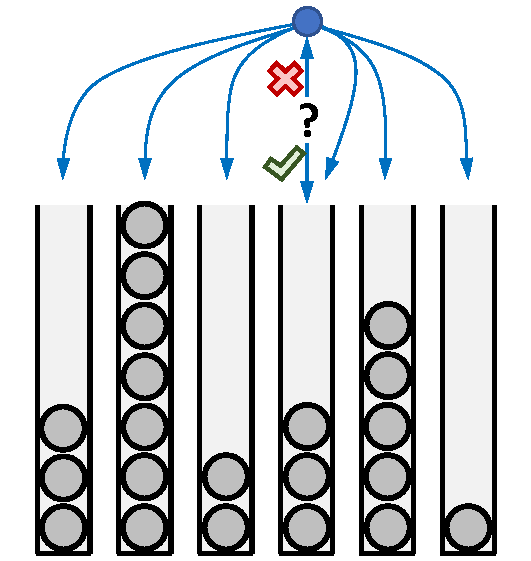
\includegraphics{Chapter1/Figs/two_thinning_intro.pdf}
    \caption{One step of the \TwoThinning protocol. The fourth bin was chosen uniformly at random, so the strategy has to decide whether to place the ball there or into a bin chosen uniformly at random.}
    \label{two-thinning-intro}
\end{figure}



\section{My approach} \label{my-approach}
For the decision strategies I compare heuristics (e.g.\ mean thinning) with strategies learnt by reinforcement learning (RL) and dynamic programming (DP) methods. RL is a natural choice, since we have to make optimal decisions (``choose optimal thresholds for accept/reject'') in a dynamic, stochastic process. RL adjusts the strategy by collecting rewards, which I will discuss in Section~\ref{dqn-implmentation-two-thinning}. RL has already been applied to load balancing, mostly related to networking~\cite{attiah2020RLcellular, yeo2021controller}, but those settings are considerably different from balls-into-bins.


The balls-into-bins protocols I will study received much attention in the academic community only recently, though there have been earlier, mostly empirical studies as well (see e.g.~\cite{derek1986twothinningfirstattempt}). At the moment, there are strategies (e.g.\ for \TwoThinning) that are proven to be asymptotically optimal, i.e., the achieved maximum load is optimal up to constant factors (for sufficiently large $n$). There are three reasons why most of these theoretical results are not applicable for small values: 1) results may only hold for ``sufficiently large'' values of balls and bins, 2) constant factors in big-Oh notation are large, 3) suggested \textit{positive} integer parameter values used by the strategy would equal to $0$, e.g.\ $\floor{\ln(\ln(\ln(\mathrm{number\ of\ servers})))}$ which is usually $0$ even for large datacentres~\cite{uzaman2019datacentresize}.


To the best of my knowledge, my work is novel in several aspects. The decision strategies I find using RL and DP are optimised for specific values of $n$ and $m$, not asymptotically. In particular, this is the first work analysing the exactly optimal strategies, which I will do using DP for moderate values of $n$ and $m$.


In a practical implementation of \TwoThinning, it is often much more natural and effective if the queried server itself decides whether to take the job, rather than sending back its current load value back to the client which makes the decision whether to accept of reject that server. Overall, the protocol is 1) the client chooses a server uniformly at random, 2) the server either completes the job or passes it on to a server chosen uniformly at random.

The servers need some ``reference'' to assess their load relative to others, which potentially requires some centralised information. There are several options, for example the servers could maintain the total number of jobs in the system, or they could synchronise their individual loads from time-to-time (see e.g.~\cite{zhang2018datacenterloadbalancing} for efficient communication in datacentres). I will focus on the latter, which crucially allows servers to make their decisions based on the (possibly slightly outdated) loads of all the other ones. When a server decides to pass on a job to another server, the motivation for choosing the other server at random is that due to parallelism and the possibly outdated information, the seemingly least loaded server could quickly become the most overloaded if all the other servers pass the jobs to that one. This project being the first work on looking for exactly optimal strategies, I will try to solve a slightly simplified but still very challenging problem, where the strategy is always given the \textbf{exact load distribution} at the moment. In practice, the solutions for this simplified problem could be used to decide on a strategy right after a synchronisation, and that strategy can be followed until the next synchronisation. I further assume that all servers use the same strategy.


Overall, the intention of this more theoretical dissertation is survey the applicability of RL and other approaches to balls-into-bins, and to gain a deeper insight into how optimal strategies look like. In the future, the insights could be fed back to building efficient, directly applicable strategies.


\section{Outline}

The outline of the dissertation is as follows.


In Chapter~\ref{preparation}, I formally define the balls-into-bins setting and the core protocols I will analyse in later chapters, and I explain the basics of RL, with particular focus on \DQL.


In Chapter~\ref{implementation}, I explain the implementation considerations of the RL and DP algorithms and discuss the other strategies, for various protocols.


In Chapter~\ref{evaluation}, I compare the implemented approaches from various aspects, also providing several insights via a thorough hyperparameter analysis for RL, and lemmas and conjectures for the DP algorithm and other strategies.

In Chapter~\ref{conclusion}, I conclude with some future work ideas for improving the RL approaches, gaining better insights to optimal strategies, and extending the study to different protocols.